\documentclass[a4paper,11pt,twoside]{scrartcl}
\usepackage[T1]{fontenc}
\usepackage{subcaption}
\usepackage[utf8]{inputenc}
\usepackage{ngerman, eucal, mathrsfs, amsfonts, bbm, amsmath, amssymb, stmaryrd,graphicx, array, geometry, color, wrapfig, float, hyperref, epstopdf,gensymb, subcaption}
\geometry{left=25mm, right=15mm, bottom=25mm}
\setlength{\parindent}{0em} 
\setlength{\headheight}{0em} 
\title{Graphentheorie\\ Blatt 1}
\author{Markus Vieth}
\date{\today}
\input{../head/lstlisting.tex}
\newcommand{\ddvec}[2]{\begin{pmatrix}#1\\#2\end{pmatrix}}
\newcommand{\dddvec}[3]{\begin{pmatrix}#1\\#2\\#3\end{pmatrix}}
\newcommand{\longvec}[1]{\overset{\longrightarrow}{#1}}
\newcommand{\eunorm}[1]{\left\lVert#1\right\rVert_2}
\newcommand{\scalar}[2]{\left<#1,#2\right>}
\begin{document}

\newcommand{\cor}[1]{\textcolor{red}{\textit{#1}}}
\maketitle
\cleardoublepage
\pagestyle{myheadings}
\markboth{Markus Vieth}{Markus Vieth}

\newpage
\section*{Aufgabe 1}
\subsection*{a}
$M \subseteq E$ heißt Matching, wenn jeder Knoten zu höchstens einer Kante aus $M$ inzident ist.
\subsection*{b}
$M$ heißt \underline{perfektes} Matching, wenn $\forall v \in V~ \exists e \in M | e = \{v,x\}$
\subsection*{c}
$M$ heißt \underline{maximales} Matching, wenn $M$ durch Hinzunahme einer weiteren Kante nicht vergrößert werden kann.
\subsection*{d}
Ein Fluss ist eine Funktion $f:E\rightarrow\mathbb{R}^+_0$ welche:
\begin{itemize}
	\item die Kapazitätsbedinung: $\forall(u,v)\in E| 0 \leq f(u,v) \leq c(u,v)$
	\item die Flusserhaltung: $\forall u \in V \setminus\{ s,t \} | \sum_{v\in V} f(u,v) = \sum_{v\in V} f(v,u)$
\end{itemize} erfüllt.\\
Der Wert eines Flusses ist dann bestimmt durch \[|f| = \sum_{v\in V} f(s,v) - \sum_{v\in V} f(v,s) = \sum_{v\in V} f(v,t) - \sum_{v\in V} f(t,v)\]
\subsection*{e}
Ein Fluss $f$ ist maximal, wenn es keinen $f$-verbessernden Pfad gibt.
\section*{Aufgabe 2}
\subsection*{a}
\begin{figure}[h]
\centering
\begin{subfigure}[b]{0.45\linewidth}
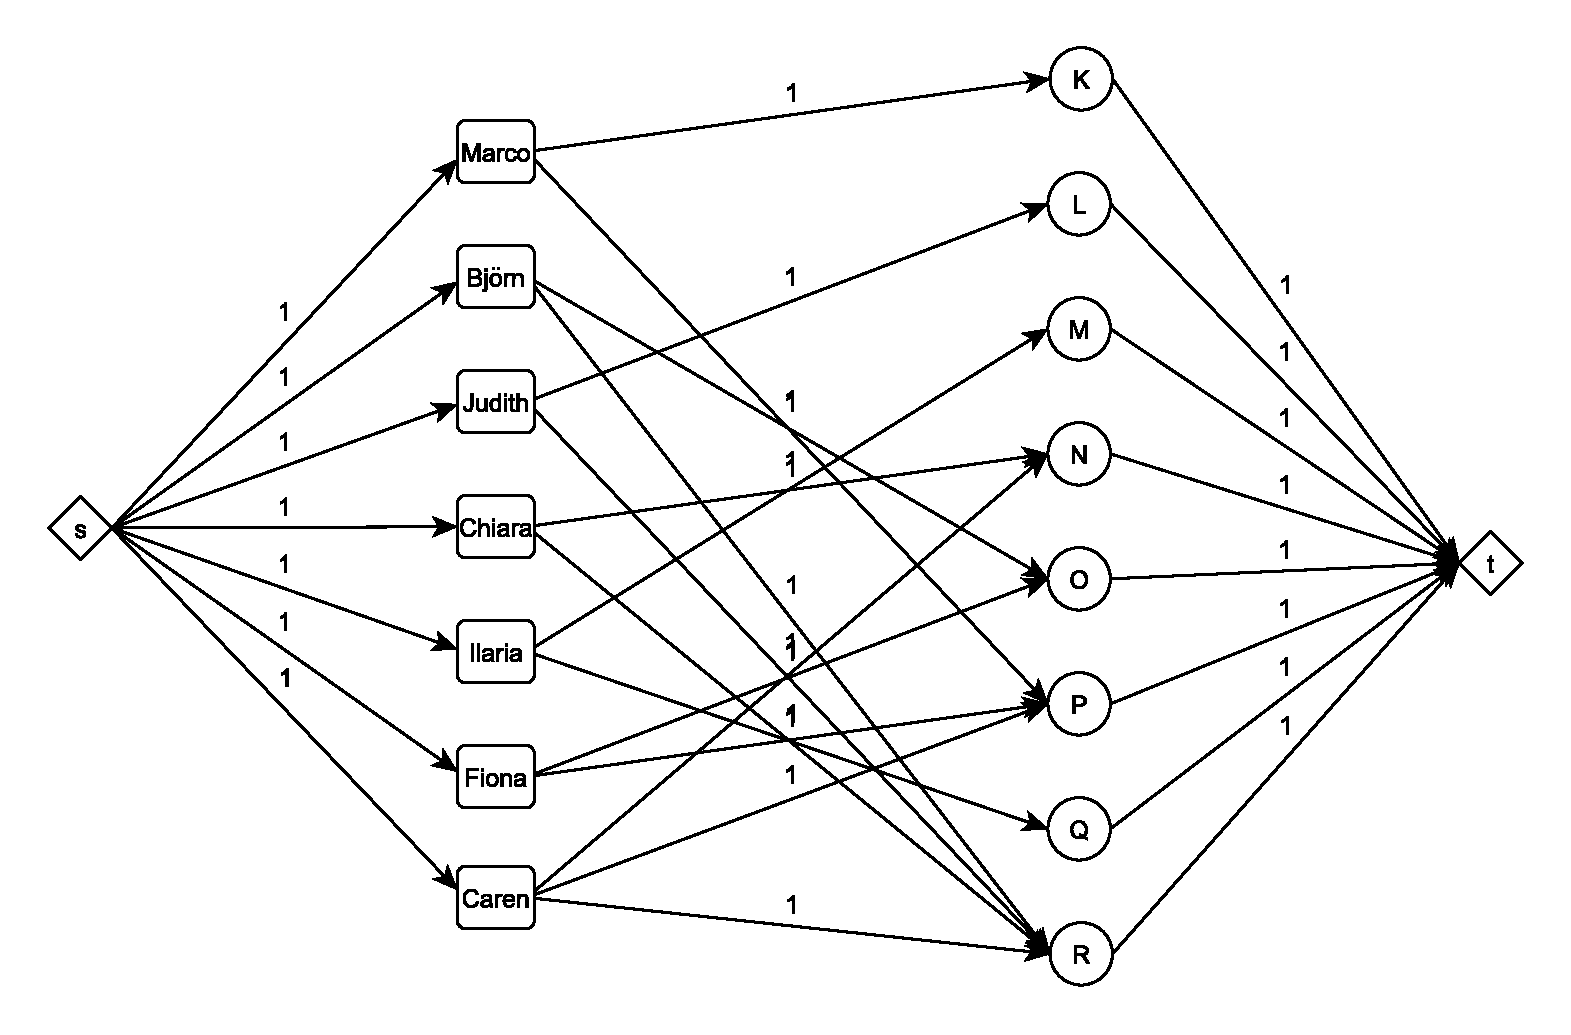
\includegraphics[width=\linewidth]{img/start}
\caption{Start}
\label{fig:start}
\end{subfigure}
~~
\begin{subfigure}[b]{0.45\linewidth}
\centering
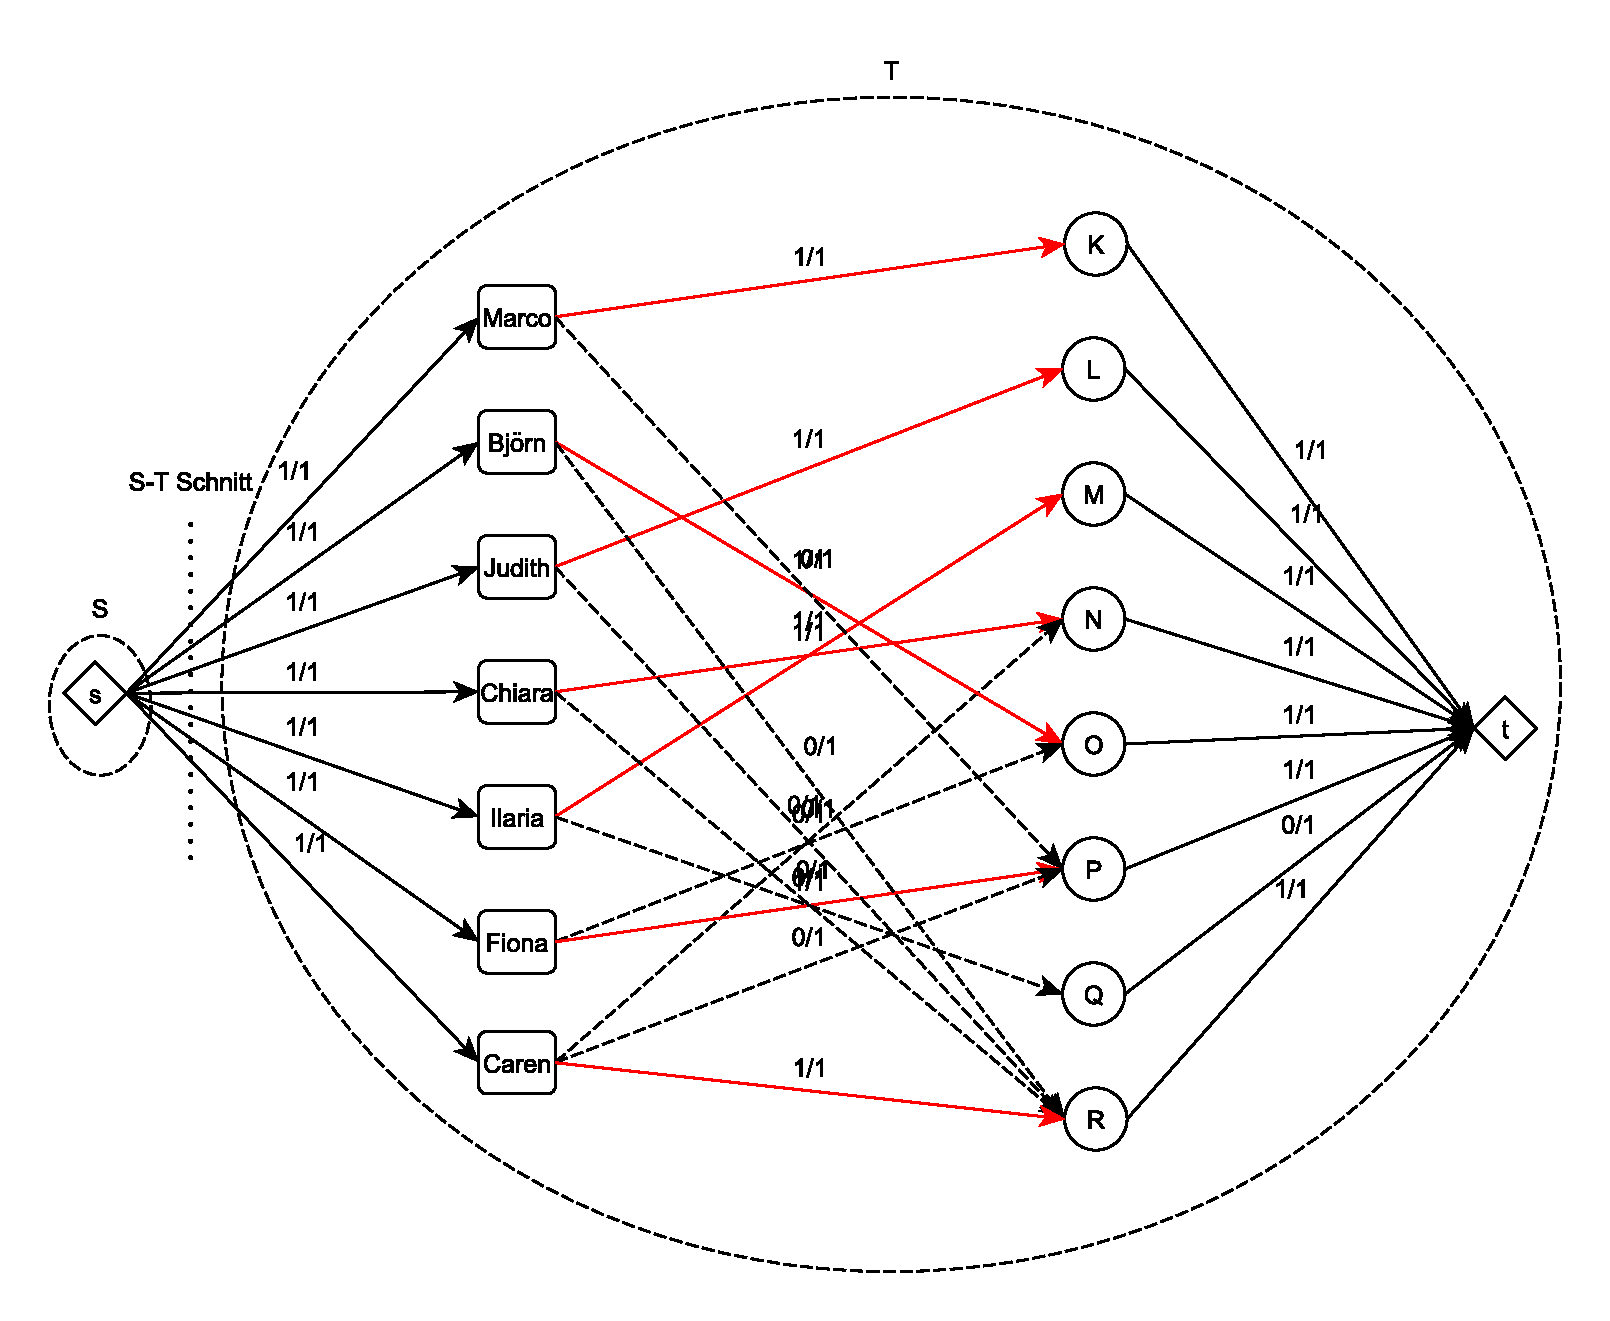
\includegraphics[width=\linewidth]{img/ende}
\caption{Ende}
\label{fig:ende}
\end{subfigure}
\end{figure}

Um zu zeigen, dass das Matching maximal ist, reicht es zu zeigen, dass der Fluss maximal ist:
\[ |f| = 7 = c(S,T) \overset{\text{Max-Flow-Min-Cut-Theorem}}{\Longrightarrow} \text{Fluss f ist maximal} \]
\begin{wrapfigure}{r}{0.45\linewidth}
\centering
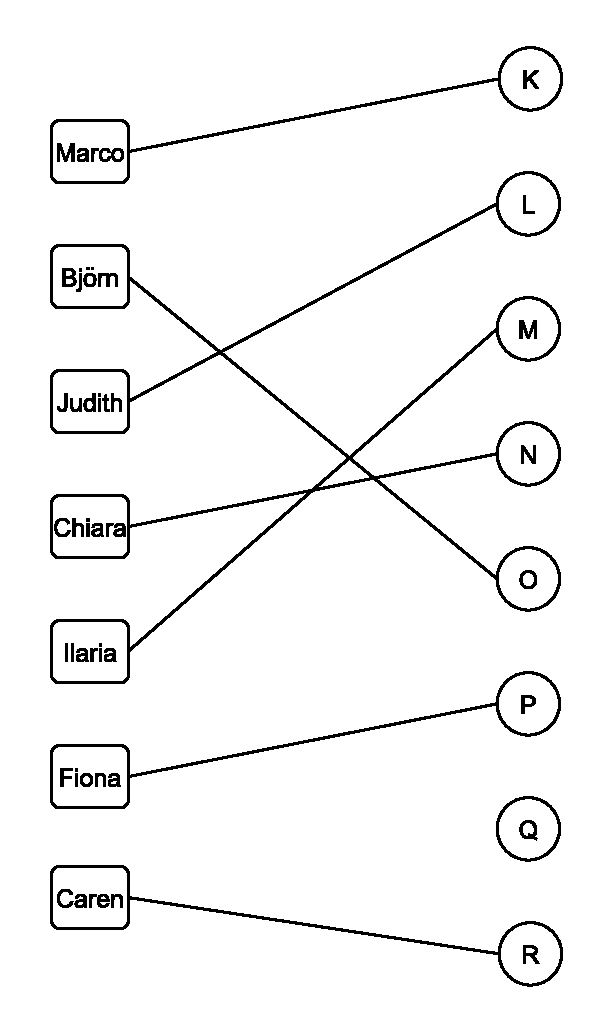
\includegraphics[width=0.9\linewidth]{img/res}
\caption{Lösung}
\label{fig:res}
\vspace*{-6em}
\end{wrapfigure}
\subsection*{b}
Es ist kein perfektes Matching möglich, da es mehr Stellen als Bewerber gibt.
\subsection*{c}
Sei $V'_{min} = \min{|V'|}$ eine minimale Überdeckung. Es gilt:
\[ |V'_{min}| \leq |E| \]
Es reicht zu zeigen:
\[ \nexists M \text{ Matching von G }| ~|M| > |V'_{min}| \]
Beweis durch Widerspruch:\\
Sei $|M| > |V'_{min}|$,
\[ \Rightarrow \exists \{u,v\} \in M | u \notin V'_{min} \land v \notin V'_{min} \]
da alle Kanten in $M$ knotendisjunkt sind, enthält eine Überdeckung mindestens einen Knoten einer jeder Kante aus $M$. Dies steht im Widerspruch zur Annahme, dass $V'_{min}$ eine Überdeckung ist.\\
$\Rightarrow~~|M| \leq |V'_{min}| \leq |V'|$ 
\subsection*{d}
Zu zeigen: Ein Baum hat höchstens ein perfektes Matching\\
Beweis durch Widerspruch:\\
Seien $M_1, M_2$ perfekte Matchings im Baum $G = (V,E)$, dann $\exists~ u \in V | \{u,v\} = e_1 \in M_1 \land \{u,w\} = e_2 \in M_2 \land e_1 \neq e_2$. Nun gilt wiederum: $\exists x,y \in V | \{ w,x \}\in M_1 \land \{ v,y \} \in M_2$. Sei $v=v_0$ und $ (M_1(v) = u \Leftrightarrow \{u,v\}\in M_1$, dann ist $(M_1 \circ M_2)(v_0) = v_2 $ das einseitige verlängern des Pfades ab $v$ durch abwechselndes hinzufügen von Kanten aus $M_1$ und $M_2$. Sei nun $ v_0, M_2(v_0), (M_1 \circ M_2)(v_0),\dots, (M_1 \circ M_2)^n(v_0)=v_{2n} $ ein Pfad in $G$. Da es keinen "`Weg"' in den Durchschnitt $M_1\cap M_2$ geben kann, gilt: $v_k \neq V_{k+2}$. Da es keine "`Sackgassen"' gibt und jeder Weg endlich sein muss, folgt: $\exists i,j \in \mathbb{N} | ~ v_i = v_j \land i < j-2$. Da $v_0, v_1, v_2$, wie vorher gezeigt, paarweise verschieden sind, existiert ein Widerspruch zur Annahme, das $G$ ein Baum und somit kreisfrei ist.\\
$\Rightarrow ~~M_1 = M_2$, es kann also maximal ein perfektes Matching in einem Baum existieren.\\

In einem Baum mit ungerader Knotenanzahl kann kein perfektes Matching existieren, da alle Kanten aus einem Matching knotendisjunkt sein müssen und da eine Kante immer aus 2 Knoten besteht, folgt dass ein Baum mit ungerader Knotenanzahl kein perfektes Matching haben kann.
\end{document}